\documentclass{article}
\usepackage{amssymb, amsthm, enumitem}
% Prevent file encoding error
\usepackage[utf8]{inputenc}
% Margin for viewing/printing aesthetics
\usepackage[margin=1in,top=0.5in,bottom=0.5in]{geometry}
% Stick to the left (question number) for all math equations
\usepackage[fleqn]{amsmath}
% Supposed to make the text look better (subjective) via reduced space between letters
% https://www.khirevich.com/latex/microtype/
\usepackage{microtype}
% For \begin{comment}...\end{comment}
\usepackage{verbatim}
% For syntax highlighting
\usepackage{minted}
\begin{comment}
Install: pip install Pygments
Add "-shell-escape", to vscode:
Open settings, search for "latex-workshop.latex.tools", click "Edit in settings.json", add "-shell-escape" to the pdflatex 
command.
\end{comment}

% For displaying accurate time
\usepackage{datetime}
% For PDF metadata
\usepackage[pdfusetitle]{hyperref}
% For PDF outline (table of contents)
\usepackage{navigator}
% Automatically add section to outline
\newcommand{\mysectionstar}[2][]{%
    \ifthenelse{\equal{#1}{}}%
        {\section*{#2}}% If optional argument is empty
        {\section*[#1]{#2}}% If optional argument is not empty
    \outline{1}{#2}%
}
\newcommand{\mysubsectionstar}[2][]{%
    \ifthenelse{\equal{#1}{}}%
        {\subsection*{#2}}% If optional argument is empty
        {\subsection*[#1]{#2}}% If optional argument is not empty
    \outline{2}{#2}%
}
\newcommand{\mysubsubsectionstar}[2][]{%
    \ifthenelse{\equal{#1}{}}%
        {\subsubsection*{#2}}% If optional argument is empty
        {\subsubsection*[#1]{#2}}% If optional argument is not empty
    \outline{3}{#2}%
}
% For images
\usepackage{graphicx}
\begin{comment}
Usage:
\begin{figure}[H]
\centering

\includegraphics[width=0.4\textwidth]{image.png}
\caption{Descriptive text for Figure}
\end{figure}
\end{comment}
% For pseudocode
\usepackage{algorithm}
\usepackage{algpseudocode}
% For scalable fonts
\usepackage{lmodern}
% For graph
\usepackage{pgfplots}
\pgfplotsset{compat=1.18}

% Independent symbol
\newcommand\independent{\protect\mathpalette{\protect\independenT}{\perp}}
\def\independenT#1#2{\mathrel{\rlap{$#1#2$}\mkern2mu{#1#2}}}

\title{Assignment template using \LaTeX}
\author{Cheng Ho Ming, Eric (3036216734) [Class Section]}
\date{\today \ \currenttime}

\begin{document}
\maketitle

\mysectionstar{Question 1}

\begin{comment}
Listing questions using enumitems
No table of contents, but automatic counting
\end{comment}
\begin{enumerate}[label=(\alph*)]
\item $\begin{aligned}[t]
E=mc^2
\end{aligned}$

\item 1
\begin{figure}[H]
\centering

\includegraphics[width=0.4\textwidth]{image.png}
\caption{A smily face}
\end{figure}
\item
    \begin{minted}[samepage]{python3}
print(chr(sum(range(ord(min(str(not())))))))
    \end{minted}
\end{enumerate}

\mysectionstar{Question 2}

\mysubsectionstar{(a)}

Lorem ipsum dolor sit amet, consectetur adipiscing elit, sed do eiusmod tempor incididunt ut labore et dolore magna aliqua.
Ut enim ad minim veniam, quis nostrud exercitation ullamco laboris nisi ut aliquip ex ea commodo consequat.
Duis aute irure dolor in reprehenderit in voluptate velit esse cillum dolore eu fugiat nulla pariatur.
Excepteur sint occaecat cupidatat non proident, sunt in culpa qui officia deserunt mollit anim id est laborum.

\newpage

\mysubsectionstar{(b)}

\mysubsubsectionstar{(i)}

The pseudocode for Euclid's algorithm is as follows:

\begin{algorithm}
\caption{Euclid's algorithm}
\text{Find the greatest common divisor of two numbers.}
\begin{algorithmic}[1]
\Procedure{Euclid}{$a,b$}
\State $r \gets a \mod b$
\While{$r \neq 0$}
\State $a \gets b$
\State $b \gets r$
\State $r \gets a \mod b$
\EndWhile
\State \textbf{return} $b$
\EndProcedure
\end{algorithmic}
\end{algorithm}

\mysubsubsectionstar{(ii)}

The Python code for the Euclid's algorithm is as follows:

\begin{minted}[samepage]{python3}
def euclid(a: int, b: int) -> int:
    r: int = a % b
    while r != 0:
        a, b = b, r
        r = a % b
    return b

print(euclid(10, 5))
\end{minted}

\mysubsubsectionstar{(iii)}

\begin{center}
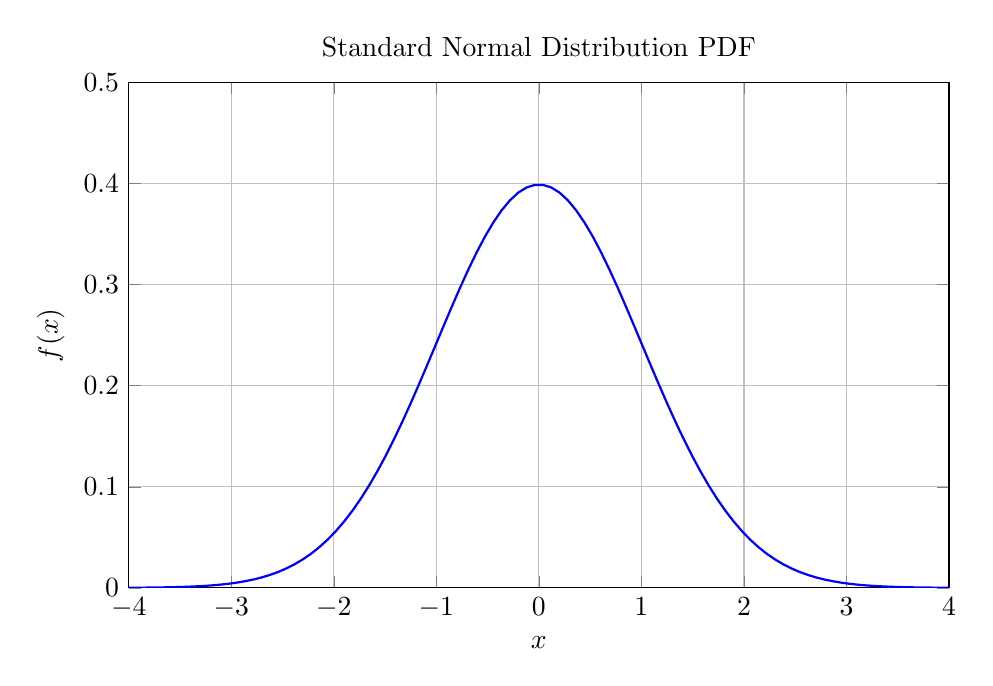
\begin{tikzpicture}
\begin{axis}[
    width=12cm,
    height=8cm,
    xlabel=$x$,
    ylabel=$f(x)$,
    title={Standard Normal Distribution PDF},
    grid=major,
    xmin=-4, xmax=4,
    ymin=0, ymax=0.5,
    samples=100,
    domain=-4:4
]
\addplot[blue, thick] {exp(-x^2/2)/sqrt(2*pi)};
\end{axis}
\end{tikzpicture}
\end{center}

\end{document}
